%usunięte z rozdziału 2
\section{Podstawowe operacje i pojęcia towarzyszące przetwarzaniu obrazów}
Choć dla człowieka informacje zawarte na obrazie są proste w interpretacji, maszyna ''widzi'' ramkę jako zwykły ciąg liczb. Dlatego aby dokonywać automatycznej detekcji pewnych zjawisk i zależności, należy poddać ją odpowiednim przekształceniom, pozwalającym wyekstrahować interesujące powiązania. Często konieczna jest także zmiana sposobu reprezentacji pikseli. Równie ważne staje się również filtrowanie zakłóceń. W książce \cite{i1823330731} opisane są najczęściej wykorzystywane algorytmy używane w takim procesie. W tej sekcji omówione zostaną te z nich, które używane są przez niektórych twórców rozwiązań z rozdziałów \ref{cha:metodyStare} i \ref{cha:analiza}. 
\subsection{Filtracja}
Filtracja obrazu ma na celu wyeliminowanie niepożądanych cech obrazu. Jest to operacja kontekstowa, a więc wymagająca informacji o jasności piksela i jego otoczenia. Staje się przez to procesem wykorzystującym duże nakłady obliczeniowe maszyny, przez co znacznie opóźnia działanie metody wykorzystującej filtrację - dlatego też istotny jest dobór jak najbardziej optymalnego sposobu eliminacji zakłóceń w zależności od danych. Dostępnych jest wiele metod, jak choćby filtracja górno- lub dolnoprzepustowa czy filtracja medianowa. Dokonuje się także klasyfikacji filtrów na liniowe (w oparciu o kombinację wartości odpowiednich pikseli obrazu wejściowego) i nieliniowe (do przekształceń wykorzystujące nieliniową funkcję odpowiednich pikseli obrazu). 
\subsubsection{Filtr medianowy}
Najczęściej używaną metodą przy usuwaniu zakłóceń typu sól i pieprz (pojedynczych pikseli o bardzo niskim/wysokim poziomie jasności) jest filtracja medianowa. W przeciwieństwie do innych rozwiązań, dokonujących najczęściej rozmycia obrazu, pozwala ona na zachowanie kształtu widocznych na scenie obiektów. Dzieje się tak między innymi dlatego, iż nie wprowadza ona do obrazu żadnych nowych wartości. Oto przykład filtracji medianowej:
\begin{figure}[!htb]
\centering
$\begin{bmatrix}
    10 & 30  & 4 \\
    20 & \textbf{0}   & 5 \\
    0  & \textbf{190} & 22 \\
    20 & 50  & 20
\end{bmatrix}$ ,
$\begin{bmatrix}
    1 & 1 & 1 \\
    1 & 1 & 1 \\
    1 & 1 & 1
\end{bmatrix}$
$\Rightarrow$
$\begin{bmatrix}
    \mathrm{x} &  \mathrm{x}  & \mathrm{x} \\
    \mathrm{x} & 10 & \mathrm{x} \\
    \mathrm{x} & 20 & \mathrm{x} \\
    \mathrm{x} &  \mathrm{x}  & \mathrm{x} 
\end{bmatrix}$
\caption{Przykładowa filtracja medianowa. Po lewej - wartości wejściowe, na środku okno filtracji, po prawej - wynik. Ponieważ operacja uwzględnia wartości sąsiedztwa, piksele brzegowe, które nie mogą być przefiltrowane w prosty sposób, oznaczone zostały jako x.}
\end{figure}
Jak widać, ponieważ pogrubione piksele reprezentowały skrajne jasności w swoim sąsiedztwie (w tym przypadku $3\times 3$), zostały podmienione wartościami mediany ze zbioru pikseli otoczenia. Wykorzystując tę metodę można odszumić nawet skrajnie zakłócony obraz. Należy jednak pamiętać, iż nadaje się ona głównie do eliminowania artefaktów typu sól i pieprz. Pozostawia także po sobie ślady w postaci ''obgryzionych'' krawędzi - niekiedy zmniejszając bądź zwiększając obszar zajmowany przez obiekty. Ważnym jest więc dobór odpowiedniego rozmiaru sąsiedztwa - większe okno wiąże się ze skuteczniejszą eliminacją zakłóceń, jednak mocno zniekształca obraz. Zwiększają się także wymagania algorytmu w kwestii obliczeniowej.
\subsection{Dylatacja}
Jednym z podstawowych przekształceń morfologicznych, czyli modyfikujących rozmiar i kształt figury na obrazie, jest dylatacja. Najczęściej wykonywana jest na obrazie binarnym. Ma ona na celu ''powiększanie'' elementów, często w celu rekonstrukcji bądź uwydatnienia pewnych ich cech.
\paragraph{}
Do wykonywania tej operacji służy \textbf{element strukturalny}, czyli pewien fragment obrazu z wyróżnionym punktem centralnym. Jest on przesuwany po całym obrazie w celu sprawdzania zgodności wzorca, a następnie podejmowana jest decyzja co do nowej wartości piksela centralnego. Jeśli którykolwiek z pikseli branych pod uwagę na podstawie szablonu elementu strukturalnego ma wartość '1', w przypadku dylatacji piksel centralny również otrzymuje wartość '1'.
\begin{figure}[!htb]
\centering


\includegraphics[width=0.4\textwidth]{img/sample}

\includegraphics[width=0.4\textwidth]{img/sample}
\caption{Dylatacja z obiektem strukturalnym 3x3. Po lewej - wejściowy obraz, po prawej - obraz po dylatacji}
\end{figure}
\subsection{Erozja}
Erozja jest niejako operacją przeciwną do dylatacji. 
%Operacją wykorzystywaną przy filtrach liniowych jest splot funkcji, czyli konwolucja. Ponieważ reprezentacja obrazów w przestrzeni cyfrowej jest dyskretna, również operacja splotu, w przestrzeni liczb rzeczywistych definiowana jako całka, może być opisana za pomocą zwykłego równania sumy:
%\begin{equation}
%\label{eq:konwolucja}
%L'(m,n) = (w x L)(m,n) = \sum_{i,j \in K} L(m-i, n-j)w(i,j)
%\end{equation}
%, gdzie L - obraz wejściowy, L' - efekt splotu obrazu z maską konwolucji, w - maska konwolucji, (m, n) - współrzędne piksela, dla którego wykonywana jest konwolucja jego otoczenia z maską w.\\
%Przykładowy splot fragmentu obrazu z maską filtru uśredniającego 3x3:
%\begin{equation}
%\label{eq:konwolucjaPrzyklad}

%\end{equation}
%\subsubsection{Normalizacja}
%Ponieważ w konwolucji wykonywane są operacje mnożenia i dodawania, otrzymane wartości mogą znacznie wykraczać poza zakres, jaki należy uzyskać w danej przestrzeni - najczęściej powinna być to liczba z przedziału [0, 255]. Jak łatwo zauważyć, w przykładzie \ref{eq:konwolucjaPrzyklad} tak właśnie się stało. W celu dostosowania uzyskanych liczb do wymaganego zakresu dokonuje się normalizacji. Jeśli w masce obecne są wyłącznie elementy nieujemne, każdy wynik konwolucji dzielony jest przez sumę jej elementów. Jeśli jednak współczynniki w macierzy w są zarówno dodatnie, jak i ujemne, normalizacja musi odbywać się według następującego wzoru:
%\begin{equation}
%L''(m,n) = \dfrac{L'(m,n)-minL'(m,n)}{maxL'(m,n)-minL'(m,n)}
%\end{equation}
\subsection{Przestrzenie barw}
\label{sec:colorSpace}
Przestrzeń barw to pewna matematyczna reprezentacja światła widzialnego w przestrzeni cyfrowej. W zależności od potrzeb stosowane są różne modele. Najpopularniejszymi są spotykane w urządzeniach elektronicznych trójkanałowe RGB (ang. \textit{Red Green Blue}) oraz komplementarny do niego, stosowany w druku CMYK (ang. \textit{Cyan Magenta Yellow blacK}), wykorzystujące właściwości ludzkiego wzroku determinujące sposób, w jaki człowiek odbiera barwy. Każdemu pikselowi obrazu są tu przypisane odpowiednie wartości na każdym kanale, na przykład czerwony piksel w reprezentacji RGB na kanale czerwonym (R) ma maksymalną wartość 255 (w 8-bitowej głębi kolorów), na niebieskim i zielonym po 0. Stosowane są one do łatwej do interpretacji przez człowieka reprezentacji cyfrowej kolorów na zdjęciach. Wprowadzają one jednak duże ograniczenia ze względu na ilość niesionej informacji. Akwizycja obrazu w innej przestrzeni pozwala na przykład na zastosowanie o wiele szerszego spektrum barw. Dlatego też często przy przetwarzaniu obrazów stosuje się inne modele, rozdzielające istotne dla maszyny informacje na oddzielne kanały, co umożliwia wydajniejsze i niekiedy dokładniejsze obliczenia na zdjęciach.
\paragraph{}
\begin{figure}[!htb]
\centering
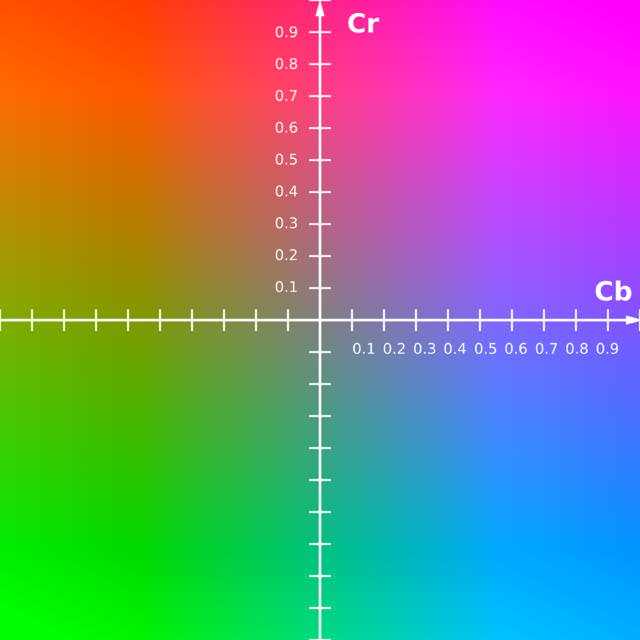
\includegraphics[width=182px]{img/YCbCr}
\caption{Reprezentacja płaszczyzny 
CbCr dla stałej luminancji Y=0.5}
%\floatfoot{Source: Wikipedia}
\end{figure}
W metodzie opisanej w rozdziale \ref{sec:BinWang}  używana jest przestrzeń YCbCr, oddzielająca kanał luminancji (Y), czyli poziomu jasności piksela, od kanałów chrominancji (Cb i Cr), przechowujących informację o jego odcieniu i nasyceniu. Taki sposób reprezentacji powstał z wykorzystaniem faktu, iż oko ludzkie jest o wiele bardziej czułe na poziom jasności obiektu, niż na jego kolor. Konwersja z przestrzeni RGB do YCbCr jest stosunkowo prosta - można ją zapisać w postaci macierzy:
%\begin{equation}

\[
\begin{bmatrix}
    Y & Cb & Cr \\
\end{bmatrix}
=
\begin{bmatrix}
    R & G & B \\
\end{bmatrix}
\begin{bmatrix}
    0.299 & -0.168935 & 0.499813 \\
    0.587 & -0.331665 & -0.418531 \\
    0.114 & 0.50059 & -0.081282 
\end{bmatrix}
\]

%\end{equation}

Ponieważ wartości na kanałach RGB mieszczą się w przedziale 0-255, po przekształceniu do przestrzeni YCbCr otrzymujemy odpowiednio wartości z przedziału [0, 255] na kanale Y oraz [-128, 127] na kanałach Cb i Cr.